\chapter{Introduction}

\section{Motivation}
% ======================================================================
% Motivation aka. "Why is what we do important?"
%
% First of all: What do we do?
% - We propose a better UQ method for FINN
%
% So I need to say why UQ is important, why FINN is a good method to build on and why the previous method is bad.
%
% But instead of saying why UQ is important in general, I should say why it is important in the context of this work.
%
% So the structure is probably as follows:
% - Context of this work
% - Why FINN is a good method for this
%     - previous methods e.g. model diffusion-sorption with sorption isotherms that are only valid for some conditions
%     - FINN is a physics-aware data-based learning method that does not have these constraints and that can learn various parts of the process and additionally provides interpretable results.
% - Why UQ is imporant here
% - What the previous method was (Bayes NN) and why it is bad (can be inaccurate and computationally expensive)
% - So these limits should be addressed by this work
%
% Main message: Why **efficient** UQ is imporant here
% --------------------------

Understanding and predicting the transport of contaminants in groundwater is paramount for effective environmental remediation and protection. Traditional modeling approaches, which rely on parametric models with few parameters fitted to data, have been shown to be more inaccurate and less generalizable \cite{finn} than machine learning based approaches. Specifically, these traditional models often fail to accurately predict contaminant concentrations, leading to unreliable estimates of groundwater quality. Furthermore, their limitations stem from the specific assumptions used in their derivation, which can be overly simplistic or restrictive, hindering their ability to capture the complexity of real-world systems and making them less effective for predicting contaminant transport in diverse environments.

The Finite Volume Neural Network (FINN) \cite{finn} offers a promising alternative, leveraging a physics-aware, data-driven approach to learn various parts of the physical process directly from experimental data. This allows for greater flexibility and interpretability compared to traditional methods. However, with the additional complexity, the propagation of uncertainty in the data through the entire process up to the output becomes more challenging. But efficient and reliable uncertainty quantification (UQ) is crucial for determining the confidence in predicted contaminant transport. Existing UQ methods for FINN, such as Bayesian Neural Networks with Markov Chain Monte Carlo (MCMC) sampling \cite{bardenet2017markov}, can be computationally demanding, limiting their practical applicability. This work addresses these limitations by proposing computationally efficient UQ methods for FINN, enabling faster and more reliable uncertainty estimation for contaminant transport predictions.


\section{Background}
The transport of contaminants in groundwater is a complex process that involves various physical and chemical interactions. One crucial aspect is diffusion-sorption, where contaminants dissolved in groundwater can interact with the solid phase of the porous medium, such as clay, leading to sorption and desorption processes. This interaction significantly affects the migration and fate of contaminants.

Traditional approaches for modeling contaminant transport rely on numerical solutions of partial differential equations (PDEs) that describe the physical processes. These PDEs often involve parameters that are difficult to measure directly, necessitating the development of parametric models based on physical principles and specific assumptions.
One key parameter in these models is the retardation factor, $R(c)$, which quantifies the effect of sorption on contaminant transport. Sorption, the process by which contaminants attach to the solid phase of the porous medium, can significantly influence the rate and extent of contaminant migration. The retardation factor is typically a function of the contaminant concentration, $c$, and depends on the specific interaction between the contaminant and the soil properties.
A common parametric model for defining $R(c)$ are sorption isotherms. Among the most frequently used are the linear, Freundlich, and Langmuir isotherms \cite{finn} (see Figure \vref{fig:parametric_isotherms}).

Determining the retardation factor from concentration data is an inverse problem. Instead of directly solving the PDE with known parameters, the goal is to infer the unknown retardation factor function ($R(c)$) from observed concentration data. This inverse problem is challenging due to the limited availability and potential noise in the data, as well as the complexity of the underlying sorption processes. Even without noise, uniqueness is not guaranteed for implicit equations. To date, we are not aware of any studies that have mathematically or empirically investigated the uniqueness of the retardation factor for the diffusion-sorption PDE given concentration data and boundary conditions. Understanding the uniqueness of the retardation factor is crucial because it significantly impacts the assessment of uncertainty. If multiple mathematically exact solutions exist, then differences between two solutions obtained by the inverse solver cannot be attributed to uncertainties in the data alone, but may reflect inherent non-uniqueness in the problem itself.

Recent advances like physics-informed neural networks in ML have opened up new possibilities for modeling complex physical systems, including contaminant transport. ML-based approaches can learn intricate relationships from data, offering potential advantages over traditional methods in terms of accuracy, flexibility, and generalizability. FINN \cite{finn} is a physics-informed ML approach that combines the strengths of traditional numerical methods with the adaptability of neural networks. FINN leverages the finite volume method to discretize the governing PDE and employs neural networks to learn the unknown or uncertain components, such as the retardation factor. This allows FINN to incorporate physical constraints and conservation laws while simultaneously learning from data.

While FINN has shown promising results in modeling contaminant transport, quantifying the uncertainty associated with its predictions remains a challenge. Existing UQ methods for FINN, such as BNNs with MCMC sampling, can be computationally demanding, limiting their practical applicability. This motivates the development of more efficient UQ methods for FINN, which is the focus of this study. Our goal is to develop computationally efficient UQ methods for estimating the uncertainty in the retardation factor predicted by FINN, enabling faster and more reliable assessment of contaminant transport predictions.

\begin{figure}[h]
    \centering
    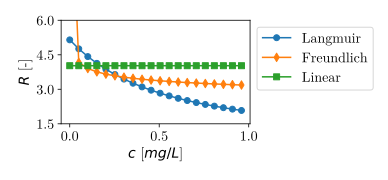
\includegraphics{figs/parametric_isotherms.pdf}
    \caption{Parametric sorption isotherms for the set of parameters used in Section \vref{sec:synthetic_data}.}
    \label{fig:parametric_isotherms}
\end{figure}


\section{Contributions of this Work}
This study addresses UQ in the FINN framework when applied to a diffusion-sorption process. We begin with an empirical analysis of the uniqueness of the retardation factor, which is a crucial step for interpreting the FINN output. We summarize FINN and PI3NN (Prediction Intervals from Three Neural Networks), the foundational methods used in this work.
A novel framework tailored for FINN called NNPIE (Neural Network Prediction Interval Estimation) is introduced to assess both aleatoric and epistemic uncertainty, allowing us to construct prediction intervals for the retardation factor.
We apply this framework to synthetic and experimental data to quantify the uncertainty of the retardation factor and compare the performance of our proposed methods against a BNN baseline employing MCMC sampling. Our results demonstrate that NNPIE provides a computationally efficient alternative to MCMC for obtaining prediction intervals for the retardation factor, offering valuable insights into the reliability of the estimated parameter.


\section{Related Work}
%=========================
% This is better but needs some work still:
% 
% Uncertainty quantification (UQ) for contaminant transport models is crucial for reliable risk assessment and decision-making. Traditional approaches often rely on computationally expensive Monte Carlo simulations [cite relevant work on MC for contaminant transport]. While Bayesian approaches offer a robust framework for UQ, applying them to complex PDEs like the diffusion-sorption equation poses challenges due to the computational cost of methods like Markov Chain Monte Carlo (MCMC) [cite BNN/MCMC for PDEs, e.g., Bardenet 2017]. Physics-informed neural networks (PINNs) [cite Raissi et al.] have emerged as a promising alternative for solving PDEs, and recent work has explored UQ in PINNs [cite examples, possibly focusing on computational efficiency challenges]. However, efficient UQ methods tailored for the specific challenges of FINN, a specialized PINN approach using the finite volume method, remain limited. This work addresses this gap by proposing computationally efficient UQ methods for FINN, drawing inspiration from techniques like PI3NN [cite PI3NN] that offer a faster alternative to traditional Bayesian methods for prediction interval estimation. This study also contributes to the broader field of inverse problems in subsurface hydrology [cite relevant reviews], where UQ plays a critical role in characterizing parameter uncertainty and its impact on predictions.
%=======================
Existing UQ methods for PDEs often rely on computationally expensive Monte Carlo simulations, limiting their applicability to complex problems. Bayesian Neural Networks, while a popular choice for UQ in deep learning, can be challenging to train and scale, particularly for high-dimensional parameter spaces. Methods like PI3NN offer a more efficient alternative for prediction interval estimation but have not yet been explored within the context of FINN. While considerable research has been dedicated to UQ in deep learning and inverse problems more broadly, efficient and scalable approaches specifically tailored for the unique challenges posed by FINN, such as those proposed in this work, remain limited. % TODO: I don't like this but better than nothing


\section{Outline of this Work}
This paper is organized as follows: Section \ref{sec:basics} introduces the diffusion-sorption equation governing contaminant transport, formalizes the inverse problem of determining the retardation factor, and reviews the FINN, PI3NN, and Bayesian neural network methodologies. We also present an empirical analysis of the uniqueness of the retardation factor inverse problem. Section \ref{sec:methodology} details our proposed Neural Network Prediction Interval Estimation (NNPIE) framework for UQ in FINN, including its variants for hyperparameter and data uncertainty. Section \ref{sec:data_and_setup} describes the synthetic and experimental datasets used for evaluation and the experimental setup. Results and discussion are presented in Section \ref{sec:results_and_discussion}, comparing NNPIE with the BNN/MCMC baseline in terms of accuracy, runtime, likelihood, and reliability. Finally, Section \ref{sec:conclusion} summarizes our findings, discusses limitations, and outlines future research directions.



\chapter{Basics}
\label{sec:basics}

\section{Problem Statement}
The diffusion-sorption process, governed by a PDE, describes contaminant transport in groundwater. Experimentally, data can be obtained from a soil cylinder, including breakthrough curves at a fixed location ($x=L$) over time ($t \in [0, T_{\text{end}}]$), and a concentration profile at a specific time ($t=T_{\text{end}}$) across the cylinder's length ($x \in [0,L]$). While a complete concentration field $c(x,t)$ (see Figure ~\vref{fig:c_diss_field_full}) would be ideal, it's practically unobtainable as measurements at all $x$ values require destructive sampling. Solving the PDE requires knowing the retardation factor, $R(c)$, which quantifies sorption and is dependent on soil properties. Since $R(c)$ is typically unknown, FINN is employed to learn it from the available data. However, uncertainties arise from measurement errors in the data and non-uniqueness of the solver solution, leading to uncertainty in the learned retardation factor. Therefore, the goal is to estimate a prediction interval around the learned $R(c)$ to quantify this uncertainty.

\begin{figure}[h]
    \centering
    \includegraphics{figs/c_diss_field_full.pdf}
    \caption{Synthetic concentration field $c(x,t)$ generated using the Langmuir isotherm for a spatial domain of $x \in [0, 1]$ meters and a temporal domain of $t \in [0, 10000]$ days.}
    \label{fig:c_diss_field_full}
\end{figure}


The diffusion-sorption Equation ~\vref{eq:diff-sorpt-pde} reads:

\begin{equation}
    \frac{\partial c}{\partial t} = \frac{D}{R(c)} \frac{\partial^2 c}{\partial x^2},
    \label{eq:diff-sorpt-pde}
\end{equation}

where $c$ is the dissolved contaminant concentration, $D$ represents the effective diffusion coefficient, $t$ is time, and $x$ is the distance along the flow path.

The following boundary conditions were considered here:

\begin{itemize}
    \item Top Boundary: At the top end of the sample where pure-phase TCE is injected, a Dirichlet boundary condition is used:

    \begin{equation}
        c|_{x=0} = c_{sol} \quad \forall t : 0 \leq t \leq T,
    \end{equation}

    where $c_{sol}$ is the solubility limit of TCE in water and $T$ is the experiment time.

    \item Bottom Boundary: At the bottom end of the sample, which is flushed with clean water, a Cauchy boundary condition is applied:

    \begin{equation}
        c|_{x=L} = \frac{D}{Q} \frac{\partial c}{\partial x} \quad \forall t : 0 \leq t \leq T,
    \end{equation}

    where $Q$ is the flow rate of the clean water and $L$ is the sample length.
\end{itemize}

The goal is to learn $\hat{R}(x,t;\theta)$ (represented by a neural network) given the data $\mathcal{D} = \{ (x_i, t_i, c_i) \}_{i=1}^N$ which consists of concentration measurements $c_i$ at spatial positions $x_i$ and temporal points $t_i$. The network needs to be trained such that the PDE solution using $\hat{R}$ minimizes the error with respect to the data.




\section{Finite Volume Neural Network (FINN)}

FINN is a specialized machine learning approach that combines the strengths of traditional numerical methods with the adaptability of neural networks to solve PDEs with unknown or uncertain components. It leverages the Finite Volume Method (FVM), dividing the problem domain into discrete control volumes. The core of FINN lies in its use of ``flux kernels'' $F_i$ – neural networks that learn how quantities flow between neighboring volumes. Specifically, each volume has a flux kernel composed of two subkernels, $f_{i-}$ and $f_{i+}$, one for each direction, which model these fluxes based on the concentrations in the volume and its neighbors. These subkernels consist of two parts: a ``stencil'' component $\varphi_N$ that approximates the FVM spatial scheme and a ``diffusivity'' component $\varphi_D$ that learns how the flow rate depends on the concentration itself:

\begin{align*}
    f_{i-} &= \varphi_D(c_i) \cdot \varphi_N(c_i, c_{i-1}) \\
    f_{i+} &= \varphi_D(c_i) \cdot \varphi_N(c_i, c_{i+1}).
\end{align*}

Furthermore, FINN employs ``state kernels'' $S_i$ that take the local concentration and calculated fluxes as input to update the concentration over time. This time evolution is governed by a Neural Ordinary Differential Equation (NODE) solver \cite{chen2019neuralordinarydifferentialequations}, a differentiable method that integrates seamlessly into the neural network training. By integrating FVM discretization, specialized neural network modules, and a NODE solver, FINN is capable of learning complex time-dependent spatial patterns while adhering to physical conservation laws and boundary conditions.



\section{Uniqueness of Inverse Problem}
\label{sec:uniqueness}

As a prerequisite for uncertainty quantification, it's crucial to investigate whether the inverse problem of determining the retardation factor, $R(c)$, from concentration data is unique. Non-uniqueness, meaning multiple possible $R(c)$ functions could produce the same concentration field, would complicate the interpretation of any UQ results. Instead of a purely theoretical analysis, we conduct an empirical investigation into the uniqueness of $R(c)$ for our specific problem.

Our approach leverages the available synthetic concentration data generated using known $R(c)$ functions (e.g., Langmuir, Freundlich, and linear isotherms). We rearrange the diffusion-sorption PDE ~\vref{eq:diff-sorpt-pde} to explicitly solve for $R(c)$:

\begin{equation}
    R(c) = D \frac{\partial^2 c}{\partial x^2} \left/ \frac{\partial c}{\partial t} \right .
    \label{eq:rearranged_pde}
\end{equation}

We then numerically approximate the first-order time derivative ($\partial c / \partial t$) and the second-order spatial derivative ($\partial^2 c / \partial x^2$) of the concentration field $c(x,t)$ using a B-spline surrogate model. This spline allows us to estimate the derivatives at any point within the spatial and temporal domain of the data.

Figure ~\vref{fig:ret_uniqueness} shows the results of this empirical uniqueness analysis for three different synthetic datasets generated using the Langmuir, Freundlich, and linear isotherms. For each case, we plot the raw $R(c)$ estimates and the binned and averaged $R(c)$ values as a function of $c$. We also include a comparison with the analytical isotherms used to generate the synthetic datasets.

\begin{figure}[h!]
    \centering
    \includegraphics{figs/ret_uniqueness.pdf}
    \caption{Empirical investigation of the uniqueness of the retardation factor $R(c)$ for three different synthetic datasets generated using the Langmuir, Freundlich, and linear isotherms. The left and top panels show the raw $R(c)$ estimates (colored circles) and the binned and averaged $R(c)$ values (black line with circle markers) as a function of $c$. The bottom-right panel compares the binned and averaged $R(c)$ values (colored circle markers) with the analytical isotherms (colored line) used to generate the synthetic datasets. Error bars indicate the standard deviation inside the bin.}
    \label{fig:ret_uniqueness}
\end{figure}

The results suggest that, for these synthetic datasets, the inverse problem of determining $R(c)$ from concentration data is largely unique, apart from minor numerical inaccuracies. The binned and averaged $R(c)$ values closely follow the trend of the analytical isotherms, indicating that our approach can recover the underlying retardation behavior with reasonable accuracy.

This empirical evidence of uniqueness provides a foundation for subsequent uncertainty quantification. It suggests that discrepancies between different $R(c)$ solutions obtained using FINN can be attributed primarily to aleatoric uncertainty (e.g., measurement noise) and epistemic uncertainty (e.g., limitations in model knowledge) rather than inherent non-uniqueness in the inverse problem itself.
% TODO: Bad that I explain these uncertainties only in the next section?




\section{Uncertainty Quantification}
There are two main aspects of UQ in this context:
\begin{enumerate}
    \item UQ for FINN output: $p(\hat{c}(x,t) | \mathcal{D})$. This represents the probability distribution of the predicted contaminant concentration $\hat{c}(x,t)$ obtained from the FINN model, given the data $\mathcal{D}$.
    \item UQ for the predicted retardation factor: $p(\hat{R}(c) | \mathcal{D})$. This is arguably more important because it represents the probability distribution of the predicted retardation factor $\hat{R}(c)$ given the data $\mathcal{D}$. This distribution helps in understanding the confidence in the estimated retardation factor.
\end{enumerate}

But there are also two types of uncertainty that have to be differentiated \cite{depeweg2018decomposition, gawlikowski2023survey}:

\begin{enumerate}
    \item Aleatoric uncertainty: This arises from inherent randomness in the data and the physical system. It is irreducible and is caused by factors such as measurement noise and variability in the system parameters.
    \item Epistemic uncertainty: This stems from limited knowledge of the model (e.g. uncertainty over its parameters). It is associated with model structure, neural network architecture, and limited training data. It quantifies the model's predictive uncertainty.
\end{enumerate}

While a clear decomposition into aleatoric and epistemic uncertainty is often challenging, as seen with methods like BNNs using MCMC, our primary focus is on quantifying the overall predictive uncertainty, which includes both components. However, our method has the added advantage of decomposing the uncertainty by design, providing a more precise and interpretable quantification of both aleatoric and epistemic uncertainties.





\subsection{Bayes Neural Networks}
\label{sec:bayes_nn}
% TODO: Maybe too detailed. Move some to appendix?
This section describes the baseline methodology used for comparison, which employs Bayesian Neural Networks and MCMC to estimate the posterior distribution of the retardation factor, $\hat{R}(c(x,t))$, parameterized by a neural network (NN). The retardation factor is a function of concentration, $c$, which itself is a function of spatial position, $x$, and time, $t$. This approach updates prior beliefs about the retardation factor based on observed data, $\mathcal{D}$.

\paragraph{Prior Distribution}

A Gaussian prior distribution, $p(\theta)$, is placed over the NN parameters $\theta$, reflecting prior knowledge or assumptions. This prior is centered on the parameters $\theta_{PT}$ of a pre-trained NN, with covariance matrix $\Sigma_p = 0.05 \, I$:


\begin{equation*}
p(\theta) = \mathcal{N}(\theta | \theta_{PT}, \Sigma_p)
\end{equation*}

\paragraph{Likelihood Function}

The likelihood function, $p(\mathcal{D} | \theta)$, quantifies the probability of observing the data $\mathcal{D}$ given a specific set of NN parameters $\theta$. We assume additive Gaussian noise with standard deviation $\sigma$ corrupts the observed concentrations. Let $c_{obs}(x,t)$ represent the observed concentration at position $x$ and time $t$, and $\hat{c}(x,t; \theta)$ the concentration predicted by the model (using a FINN solver with $\hat{R}(c(x,t);\theta)$). The likelihood is:

\begin{equation}
p(\mathcal{D} | \theta) = \prod_{(x_i, t_i, c_i) \in \mathcal{D}} \frac{1}{\sqrt{2\pi \sigma^2}} \exp \left( -\frac{(c_i - \hat{c}(x_i, t_i; \theta))^2}{2\sigma^2} \right)
\label{eq:likelihood}
\end{equation}

\paragraph{Posterior Distribution}

Bayes' theorem provides the posterior distribution of the NN parameters given the data:


\begin{equation*}
p(\theta | \mathcal{D}) \propto p(\mathcal{D} | \theta) p(\theta)
\end{equation*}

\cite{finn} compare several methods to obtain samples from this distribution, including the Metropolis-Hastings algorithm, the MALA algorithm, and the Barker method. The accepted samples $\{\theta_i\}$ from the used algorithm are then treated as draws from the posterior distribution $p(\theta | \mathcal{D})$.

\paragraph{Posterior of Retardation Function}

Finally, the posterior distribution of the retardation factor $\hat{R}(c)$ is obtained by evaluating the NN with the sampled parameters $\{\theta_i\}$:

\begin{equation*}
\{\hat{R}(c | \theta_i)\} \sim p(\hat{R}(c) | \mathcal{D})
\end{equation*}

This set of retardation factor samples provides a probabilistic description of the retardation behavior, incorporating the uncertainty arising from the limited and noisy data.

Since \cite{finn} obtain the best results with the Barker method and no burn-in period by starting from the pre-trained model, we follow their approach to have a fair comparison.




\subsection{PI3NN (Prediction Intervals from Three Neural Networks)}
PI3NN \cite{pi3nn} is a method for constructing prediction intervals (PIs) that uses three independently trained neural networks. It aims to provide tight, non-crossing PIs across various confidence levels without requiring retraining for each level.

The method's theoretical foundation lies in approximating the ground-truth PI bounds with a family of neural networks. Specifically, PI3NN approximates the median of the target variable, $M[y]$, and the expected deviations above and below the median, $E[(y - M[y]) \ind{y-M[y]>0}]$ and $E[(M[y] - y) \ind{M[y]-y>0}]$, respectively, using three independently trained neural networks ($f_w(x)$, $u_\theta(x)$, and $l_\epsilon(x)$). These networks are trained using the standard mean squared error loss, simplifying the training process and avoiding the need for specialized loss functions and sensitive hyperparameters that often require fine-tuning in other PI methods.

Once trained, PI3NN constructs the PI bounds as linear combinations of the three networks' outputs. The coefficients of these linear combinations ($\alpha$ and $\beta$) are determined through a root-finding algorithm that ensures the desired PICP (Prediction Interval Coverage Probability) for a given confidence level $q$ ($\gamma$ in \cite{pi3nn}). This process allows for calculating PIs for multiple confidence levels without retraining the networks, offering significant computational advantages.


Figure ~\vref{fig:3pinn_illustration} illustrates the 6-step breakdown of the PI3NN process:
\begin{enumerate}
    \item \textbf{Learn the mean:} Train a neural network to approximate the mean of the target data.
    \item \textbf{Estimate the median:} Calculate the median by shifting the learned mean.
    \item \textbf{Calculate and split residuals:} Compute the residuals between the actual data and the estimated median, then separate these into positive and negative residuals.
    \item \textbf{Learn residuals:} Train two more neural networks, one to approximate the positive residuals and the other to approximate the negative residuals.
    \item \textbf{Construct PI:} Calculate a PI using the learned median and the learned positive and negative residuals.
    \item \textbf{Generate multiple PIs:} Use a root-finding algorithm to compute PIs for different confidence levels $q$ without retraining the networks.
\end{enumerate}


\begin{figure}[h]
    \centering
    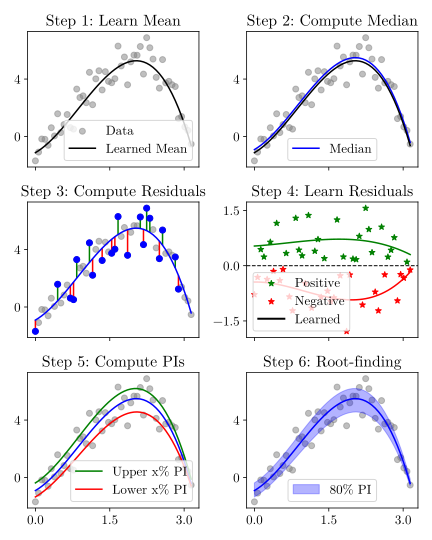
\includegraphics{figs/3pinn_illustration.pdf}
    \caption{Illustration of the PI3NN method.}
    \label{fig:3pinn_illustration}
\end{figure}





\chapter{Methodology}
\label{sec:methodology}
% TODO: Check if the math adds up here and if there are any inconsistencies.
\section{NNPIE (Neural Network Prediction Interval Estimation)}
Our objective is to determine the posterior predictive distribution $p(\hat{R}(c; \theta) = R(c)| \mathcal{D})$, which represents the probability of computing a specific retardation factor value $R(c)$ for a given concentration $c$, based on the observed breakthrough curve data $\mathcal{D}$. We present a method that computes this distribution by marginalizing over uncertain factors, denoted by $\mathcal{X}$, of the model and employing an approximate likelihood function $p(\mathcal{D} | \mathcal{X})$.

\subsection{Approximating the Posterior Predictive Distribution via Marginalization over Uncertain Factors}

\paragraph{Model Formulation}

We represent our neural network as $\hat{R}(c; \theta)$, where $c$ is the input concentration and $\theta$ denotes the network's parameters (weights and biases). The parameters $\theta$ are determined by a deterministic solver $S(h, \mathcal{D})$, which takes hyperparameters $h$ and training data $\mathcal{D}$ as input. A prior distribution $p(\mathcal{X})$ is assigned over $\mathcal{X}$; the exact form of $p(\mathcal{X})$ is not crucial for the derivation, as it suffices to generate samples from it.
When we choose to treat $h$ or the training data $\mathcal{D}$ to be a random variable, so to be our uncertain factor $\mathcal{X}$, the network parameters $\theta = S(h, \mathcal{D})$ become a random variable and thus uncertain. We denote this by $\theta_{\mathcal{X}}$ This allows us to calculate the posterior predictive distribution as follows:

\begin{align*}
p(\hat{R}(c; \theta_{\mathcal{X}}) = R(c)| \mathcal{D}) &= \int p(\hat{R}(c; \theta_{\mathcal{X}}) = R(c) | \mathcal{X}, \mathcal{D})\; p(\mathcal{X} | \mathcal{D}) \, d\mathcal{X} \\
                                          &= \int p(\hat{R}(c; \theta_{\mathcal{X}}) = R(c) | \mathcal{X}, \mathcal{D})\; p(\mathcal{X}) \underbrace{\frac{p(\mathcal{D} | \mathcal{X}) }{p(\mathcal{D})}}_{= w(\mathcal{X})} \, d\mathcal{X} \\
                                          &= \int p(\hat{R}(c; \theta_{\mathcal{X}}) = R(c) | \mathcal{X}, \mathcal{D})\; p(\mathcal{X})\; w(\mathcal{X}) \, d\mathcal{X} \\
                                          &= \int \delta(\hat{R}(c; \theta_{\mathcal{X}}) - R(c))\; p(\mathcal{X})\; w(\mathcal{X}) \, d\mathcal{X} \\
\end{align*}

The first step is the marginalization over $\mathcal{X}$, the second the application of Bayes' Theorem, and the last stems from the fact that the solver is deterministic given $\mathcal{X}$ and $\mathcal{D}$ and thus the distribution becomes a delta distribution.


\paragraph{Importance Sampling}

Sampling from $p(\hat{R}(c; \theta_{\mathcal{X}}) = R| \mathcal{D})$ is equivalent to sampling from $p(\mathcal{X})$, evaluating the solver to obtain the model parameters $\theta_{\mathcal{X}}$, evaluating the model $\hat{R}(c; \theta_{\mathcal{X}})$, and reweighting the samples with $w(\mathcal{X})$. This is the concept of importance sampling. To approximate the distribution, we draw $M$ samples $\{\mathcal{X}_m\}_{m=1}^M$ from the prior distribution $p(\mathcal{X})$ and calculate the importance weight for each:

\begin{equation*}
w_m = \frac{p(\mathcal{D} | \mathcal{X}_m)}{p(\mathcal{D})} \propto p(\mathcal{D} | \mathcal{X}_m)
\end{equation*}

As $p(\mathcal{D})$ is a constant, it can be omitted, and the weights can be normalized subsequently.


\paragraph{Likelihood Computation}

We use the same assumption about our data that the Bayesian baseline uses, which results in an easy computation of the likelihood by substituting $\theta$ with $\theta_{\mathcal{X}}$ in Equation ~\vref{eq:likelihood}:

\begin{equation*}
p(\mathcal{D} | \mathcal{X}) = \prod_{x_i, t_i, c_i \in \mathcal{D}} \frac{1}{\sqrt{2\pi \sigma^2}} \exp \left( -\frac{(c_i - \hat{c}(x_i, t_i; \theta_{\mathcal{X}}))^2}{2\sigma^2} \right)
\end{equation*}

\subsection{NNPIE Variants: Hyperparameter (Hy) and Data (Da) Marginalization}

The generalized framework above can be applied to different sources of uncertainty. Here, we describe two variants:

\paragraph{Hy-NNPIE}

In this case, we consider the uncertain factor $\mathcal{X}$ to be the hyperparameters $h$ of the solver. This variant, which we refer to as SPAN, captures epistemic uncertainty arising from the choice of hyperparameters. The equations above are applied directly with $\mathcal{X} = h$.

\subparagraph{Hyperparameter Sampling and Rationale}
The following hyperparameters were selected for perturbation in the SPAN framework to assess their influence on model output uncertainty. Each hyperparameter was chosen based on its inherent uncertainty or significant impact on the training process:

\begin{itemize}
    \item \textbf{Weight Initialization Seed:} This hyperparameter dictates the initial conditions for the neural network training process. It influences various stochastic elements, including random number generation within algorithms and the initialization of network weights. We employed the Kaiming Uniform initialization scheme \cite{he2015delving}, which mitigates the vanishing/exploding gradient problem in deep networks by ensuring consistent variance of activations and gradients throughout the network. \textit{Rationale:} The initialization of a neural network is a critical step, and the seed provides the starting point for optimization. Since a zero initialization is often detrimental, a random value is typically chosen. The impact of this fundamental choice on model output is important to quantify. Seed values were sampled uniformly from the integer range $[0, 10^9]$.
    \item \textbf{Number of Epochs:} This parameter determines the number of complete passes the model makes over the training dataset during optimization. \textit{Rationale:}  Determining the optimal number of training epochs for a neural network is often challenging. While monitoring loss is a common practice, loss can sometimes decrease unexpectedly after long plateaus. This implies that the ideal stopping point is inherently uncertain. Additionally, selecting an inadequate number of epochs can mimic the effect of a poorly chosen learning rate. A learning rate that is too high may prevent convergence to the optimal solution, similar to stopping the training process prematurely. By varying the number of epochs, we can capture this uncertainty and its effect on the model's final predictions. The number of epochs was sampled uniformly from the integer range $[10, 30]$.
    \item \textbf{MSE Loss Factor ($a_{MSE}$):} This factor weighs the contribution of the mean squared error (MSE) loss between the predicted concentration ($\hat{c}$) and the true concentration ($c$) in the overall loss function. The loss function is defined as: $a_{MSE} \cdot MSE(c, \hat{c}) + a_{Phys} \cdot Loss_{Phys}(\hat{R}(c))$. \textit{Rationale:} The optimal balance between the data-driven MSE loss and the physics-informed loss (described below) is often unknown a priori. There is no established theoretical framework to guide the selection of this factor, making it a source of uncertainty. Thus, by perturbing $a_{MSE}$, we investigate how the model's sensitivity to data fidelity influences its predictions. The values for $a_{MSE}$ were sampled from a log-uniform distribution within the range $[10^2, 10^8]$.
    \item \textbf{Physical Loss Factor ($a_{Phys}$):}  This parameter, analogous to the MSE loss factor, governs the weight of the physics-informed loss term, $Loss_{Phys}(\hat{R}(c))$, in the overall loss function. \textit{Rationale:} Similar to the MSE loss factor, the optimal weighting for the physics-informed loss is generally unknown and lacks a strong theoretical basis. By varying $a_{Phys}$, we explore how strongly the model relies on the underlying physical constraints and how this affects its predictions. The values for $a_{Phys}$ were also sampled from a log-uniform distribution within the range $[10^2, 10^8]$.
\end{itemize}



\paragraph{Da-NNPIE}

Alternatively, we can consider the uncertain factor $\mathcal{X}$ to be the dataset $\tilde{\mathcal{D}}$ itself. This variant, which we call Da-NNPIE, captures aleatoric uncertainty stemming from the inherent randomness in the data. The equations are applied with $\mathcal{X} = \tilde{\mathcal{D}}$.


\subparagraph{Mask-based Random Dataset Sampling}

To create variations in the training data, we employed a random masking technique. For each sample, a unique seed was used to randomly select 50\% of the data points for masking to generate a random dataset. ``Masking'' in this context means that these data points were excluded when computing the loss during training. Each data point had an equal probability (0.5) of being masked or retained. The seed values were drawn uniformly from the integer range $[0, 10^9]$. Figure ~\vref{fig:training_data_mask} illustrates an example of the full synthetic concentration training data with 50\% of the data points randomly masked.

\begin{figure}[h!]
    \centering
    \includegraphics{figs/c_diss_field_train_random_subset.pdf}
    \caption{Full synthetic concentration training data where 50\% of datapoints are randomly masked (dark patches).}
    \label{fig:training_data_mask}
\end{figure}


\subparagraph{Noise-based Random Dataset Sampling}

Another approach to generating dataset variations involved the introduction of additive Gaussian noise. Following \cite{nowak2016entropy}, which suggests measurement error can be modeled as Gaussian with zero mean and a standard deviation of 5\% of the measured value, we used this noise level to simulate data uncertainty comparable to experimental data.
A unique seed, uniformly sampled from the integer range $[0, 10^9]$, was used to generate the noise for each dataset. % TODO: correct reference?


\subparagraph{PI3NN-based Random Dataset Sampling}
\label{sec:random_dataset_sampling}
To generate random datasets for Da-NNPIE, we leverage PI3NN, applying it to the original breakthrough curve (BTC) dataset of core 2 $\mathcal{D}_{\text{BTC-2}}$. For more detailed information about the data, see Section \vref{sec:experimental_data}.
Let $\hat{c}(x=L, t; \theta_{\mathcal{D}_{\text{BTC-2}}})$ be the mean concentration curve predicted by FINN trained on $\mathcal{D}_{\text{BTC-2}}$, with $\theta_{\mathcal{D}_{\text{BTC-2}}}$ representing the learned FINN parameters. This FINN-predicted mean curve is used as input to the PI3NN algorithm, as it provides a more accurate representation of the underlying process compared to the mean curve learned by a standard MLP within the PI3NN framework.

PI3NN then learns the residuals, effectively modeling the distribution of $c$ given $t$. Let $F^{-1}(q | t)$ denote the quantile function predicted by PI3NN, where $q \in [0, 1]$ is the quantile level and $t$ is the time point. This function provides the concentration value at time $t$ corresponding to the $q$-th quantile of the learned distribution (see Figure ~\vref{fig:btc_dataspan_quantiles}).

To create a random dataset sample $\tilde{\mathcal{D}}(q)$, we sample a quantile level $q$ from a uniform distribution $\mathcal{U}(0, 1)$. Then, the random dataset sample is constructed as:

$$
\tilde{\mathcal{D}}(q) = \{ (t_i, F^{-1}(q | t_i) ) \}_{i=1}^N
$$

This process is repeated $M$ times to obtain a collection of random datasets $\{\tilde{\mathcal{D}}_j\}_{j=1}^M$. Each $\tilde{\mathcal{D}}_j$ is then used to train a separate instance of FINN, effectively providing a set of retardation factor samples, analogous to the samples obtained from the hyperparameter perturbation approach.

To enhance the accuracy of the likelihood computation in Section \vref{sec:likelihood}, we intentionally include the quantile levels $0$ and $1$ in the random samples. This improves the fit of the distribution to the histogram of the samples.

\begin{figure}[h]
    \centering
    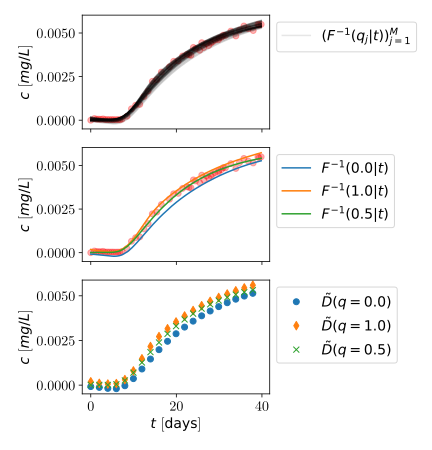
\includegraphics{figs/btc_dataspan_quantiles.pdf}
    \caption{Left: BTC quantile functions for all quantile samples $q_j$. Middle: BTC quantile functions for quantiles $0$, $0.5$, and $1$. Right: BTC datasets for quantiles $0$, $0.5$, and $1$.}
    \label{fig:btc_dataspan_quantiles}
\end{figure}



\paragraph{HyDa-NNPIE}

We can even treat both the hyperparameters and the training dataset as random variables at the same time and obtain a combined result. So $\mathcal{X} = (h, \mathcal{D})$ and both are sampled independently.

For both hyperparameter and dataset sampling, a few samples resulted in FINN not converging during training. These samples were discarded from further analysis. Convergence was determined by monitoring the loss value, requiring it to fall below a threshold of 1e-5 and remain unchanged for a certain number of iterations.


\chapter{Data and Setup}
\label{sec:data_and_setup}
\section{Environment Setup}
The experiments were conducted using Python 3.11.3. Modified versions of the FINN code from \cite{finn} and the PI3NN code from \cite{pi3nn} were used. The code and specific library versions are available on GitHub. GNU parallel \cite{tange_2023_10199085} was used for parallel execution of experiments. % TODO: insert github link

Simulations and timing measurements were conducted on a M1 Pro Macbook. This setup provided the necessary computational resources for efficient model training and evaluation.


\section{Data}
\subsection{Synthetic Data}
\label{sec:synthetic_data}
For the synthetic datasets, we used the exact parameter values from \cite{finn} (Table 1), including porosity, effective diffusion coefficient, and others. The concentration data was generated using the same solver employed by FINN, ensuring consistency in our experimental setup.


\subsection{Experimental Data}
\label{sec:experimental_data}

This study utilizes experimental data originally presented by \cite{nowak2016entropy} and subsequently employed by \cite{finn}. The data consist of breakthrough curves (BTCs) and a concentration profile, obtained from laboratory column experiments. These are detailed below and summarized in Table \vref{tab:experimental_data}.

\begin{itemize}
    \item \textbf{Core 1:} BTC data representing the concentration, $c$, at the outlet ($x = L$) of the column over time, $t$. Measurements were taken at $L = 0.0254\,\text{m}$, with time points spanning $t \in \{0.792\,\text{days} \cdot i \mid i = 0, \dots, 49\}$ (see Figure \vref{fig:core_data}, left).
    \item \textbf{Core 2:} BTC data similar to Core 1, but with $L = 0.026\,\text{m}$ and time points $t \in \{0.737\,\text{days} \cdot i \mid i = 0, \dots, 54\}$ (see Figure \vref{fig:core_data}, middle).
    \item \textbf{Core 2B:} Concentration profile data representing $c$ as a function of distance, $x$, along the column at a fixed time $T = 48.88\,\text{days}$. Measurements were taken at intervals of $0.00362\,\text{m}$, spanning $x \in \{0.00362\,\text{m} \cdot i \mid i = 0, \dots, 29\}$ (see Figure \vref{fig:core_data}, right).
\end{itemize}

\begin{table}[h!]
    \centering
    \caption{Summary of Experimental Data}
    \label{tab:experimental_data}
    \begin{tabular}{llll}
        \toprule
        Core   & Type       & Variables                 & Parameter Values                                      \\
        \midrule
        Core 1 & BTC        & $c(x=L, t)$              & $L = 0.0254\,\text{m}$, $t \in \{0.792\,\text{days} \cdot i \mid i = 0, \dots, 49\}$ \\
        Core 2 & BTC        & $c(x=L, t)$              & $L = 0.026\,\text{m}$, $t \in \{0.737\,\text{days} \cdot i \mid i = 0, \dots, 54\}$  \\
        Core 2B & Profile    & $c(x, t=T)$              & $T = 48.88\,\text{days}$, $x \in \{0.00362\,\text{m} \cdot i \mid i = 0, \dots, 29\}$ \\
        \bottomrule
    \end{tabular}
\end{table}

Following the approach of \cite{finn}, Core 2 was used for model training, while Core 1 and Core 2B served as independent test datasets. The parameter values provided alongside the concentration data in \cite{nowak2016entropy} were also used.


\begin{figure}[h]
    \centering
    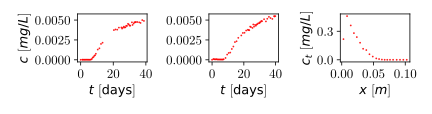
\includegraphics{figs/core_data.pdf}
    \caption{Experimental concentration data obtained from the ``Core 1'', ``Core 2'', and ``Core 2B'' sample (left to right) by \cite{nowak2016entropy}.}
    \label{fig:core_data}
\end{figure}



\section{Training Details}
The architecture and training is consistent with \cite{finn}. For the dissolved concentration $c$, the module $\varphi_D(c)$ is defined as a feedforward neural network with a 5-layer configuration of [1, 10, 20, 10, 1] neurons. For the total concentration $c_t$, $\varphi_D(c_t)$ is defined as a scalar parameter to learn the unknown diffusion coefficient $D$. Although the FINN framework allows for learning the stencil, we did not utilize this feature here.

The L-BFGS optimizer \cite{malouf2002comparison} with a learning rate of $0.1$ was used.

During training, runs were discarded if the normalized mean squared error (NMSE) on the training set exceeded $10^{-5}$. This threshold ensures a minimum level of accuracy in the learned retardation factor.


\begin{equation*}
    \text{NMSE}(y, \hat{y}) = \text{MSE}(y, \hat{y}) / \text{mean}(y)
\end{equation*}




\chapter{Results and Discussion}
\label{sec:results_and_discussion}
% TODO: I think I did not explain anywhere, why I did synth data experiments even.

\section{Synthetic Data Case}
\subsection{Hy-NNPIE}
We developed and validated our method using synthetic data prior to its application on experimental data, where actual comparisons and quantifications could be performed. As a result, our initial evaluation focused on a simplified parameter space, with only a single hyperparameter, namely the weight initialization seed.
The number of samples varied and is indicated in the respective figure captions for clarity and comparison within those specific contexts.

The influence of the seed is relatively small as can be seen in Figure \vref{fig:synthetic_SPAN_seed}.


\begin{figure}[h]
    \centering
    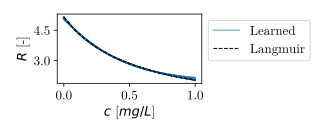
\includegraphics{figs/finn_synthetic_SPAN_seed.pdf}
    \caption{Retardation factors learned by FINN with random weight initialization seed samples and dataset generated by Langmuir isotherm (16 samples).}
    \label{fig:synthetic_SPAN_seed}
\end{figure}



\subsection{Da-NNPIE}
When applying gaussian noise of the same strength as the experimental data has, the variation in learned retardation factors becomes much larger compared to Hy-NNPIE as can be seen in Figure ~\vref{fig:synthetic_SPAN_noise}.

\begin{figure}[h]
    \centering
    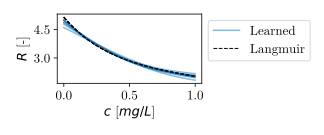
\includegraphics{figs/finn_synthetic_SPAN_noise.pdf}
    \caption{Retardation factors learned by FINN on synthetic dataset (generated by Langmuir isotherm) pertubed by gaussian noise (20 samples).}
    \label{fig:synthetic_SPAN_noise}
\end{figure}


Masking the training data has a smaller effect, as seen in Figure \vref{fig:synthetic_SPAN_losspattern}, although there is one outlier retardation factor, indicating, that there is the potential for high variations similarly to applying gaussian noise. More samples would be needed to confirm this.

\begin{figure}[h]
    \centering
    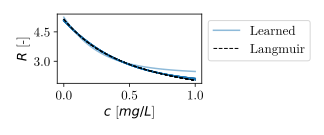
\includegraphics{figs/finn_synthetic_SPAN_losspattern.pdf}
    \caption{Retardation factors learned by FINN on synthetic dataset (generated by Langmuir isotherm) with 50\% of training data randomly masked (16 samples).}
    \label{fig:synthetic_SPAN_losspattern}
\end{figure}






\section{Experimental Data Case}

\subsection{Hy-NNPIE}
For the experimental data, the full set of hyperparameters was used: \textbf{Weight Initialization Seed}, \textbf{Number of Epochs}, \textbf{MSE Loss Factor}, \textbf{Physical Loss Factor}.

To introduce greater variability in the retardation factor output, we simultaneously sampled all hyperparameters, as opposed to the individual approach used in the synthetic data case. To still assess the impact of each hyperparameter, we conducted a sensitivity analysis, which is presented in Section \vref{sec:sensitivity}. This experiment generated a dataset of $780$ samples, based on the defined hyperparameter ranges, and the results are illustrated in Figure ~\vref{fig:span_samples}.

\begin{figure}[h]
    \centering
    \includegraphics{figs/finn_span_samples.pdf}
    \caption{Retardation samples and correspoding concentration curves obtained via FINN by training with random hyperparameters.}
    \label{fig:span_samples}
\end{figure}

% TODO: I forgot ~ for a few vrefs. (What does that even do? print the page number? Maybe I shouldn't use it everywhere then.)


\paragraph{Sensitivity Analysis}
\label{sec:sensitivity}
Sensitivity analysis investigates how variations in input parameters affect the model output. Unweighted Hy-NNPIE samples inherently perform sensitivity analysis because each sample represents a different set of hyperparameters, and the resulting retardation factor and its impact on the concentration field demonstrate the influence of those hyperparameters.

One sensitivity analysis method is based on standardized regression coefficients, sometimes referred to as beta coefficients or beta weights. They represent the relative importance of each predictor variable (hyperparameter $h$ in this case) in explaining the variance of the outcome variable ($R(c)$).
Importantly, the sum of these normalized coefficients can exceed 1 as parameters may explain common variances. The value shows how important the respective parameter is in relation to the rest.
Since these parameters are based on linear regression, they should be interpreted with caution, especially when non-linear relationships exist between the hyperparameters and the retardation factor. % TODO: reference for beta coefficients

We average the importance for $R(c)$ over a set of $c$ values and obtain $0.033$ for \textbf{Physical Loss Factor}, $0.051$ for \textbf{Weight Initialization}, $0.159$ for \textbf{MSE Loss Factor}, and $0.570$ for \textbf{Number of Epochs}.

This indicates that \textbf{Number of Epochs} and \textbf{MSE Loss Factor} have the largest impact on $R(c)$ overall. The seed used for weight initialization and the physical loss factor play only negligible roles.

Figure ~\vref{fig:sensitivity} shows the relative importance for values of $c$ over which the average was taken.

\begin{figure}[h]
    \centering
    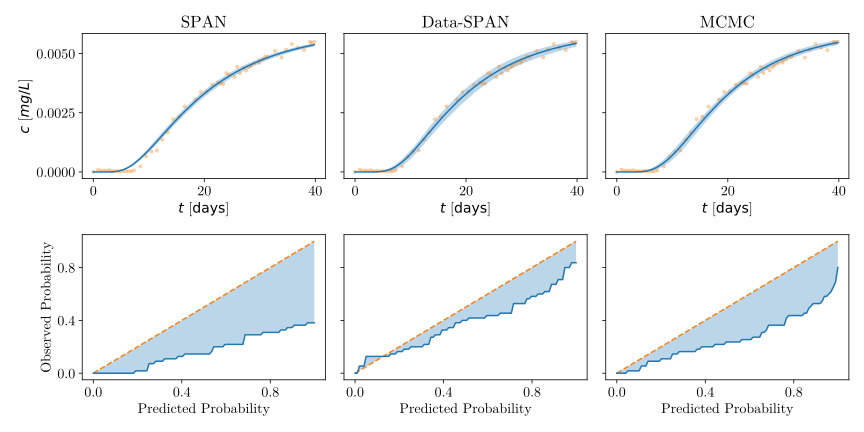
\includegraphics{figs/sensitivity.pdf}
    \caption{Relative importance on the variance of $R(c)$ of each hyperparameter for different values of $c$.}
    \label{fig:sensitivity}
\end{figure}




\subsection{Da-NNPIE}
This approach was applied only to the experimental data because the synthetic training data lacks noise, leading to extremely small residuals and a very narrow distribution that does not impact sampling. % TODO: Bit weird intro

For the experimental data, we sampled $70$ quantiles as detailed in Section ~\vref{sec:random_dataset_sampling}. The results are shown in Figure ~\vref{fig:dataspan_samples}.


\begin{figure}[h]
    \centering
    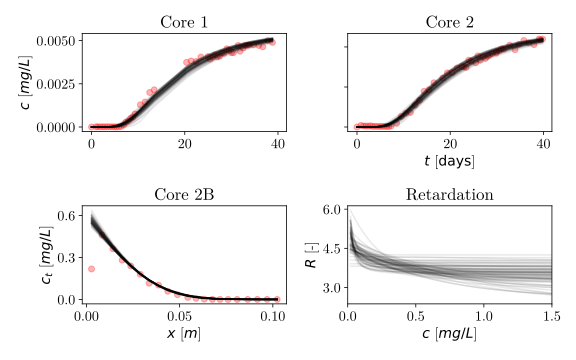
\includegraphics{figs/finn_dataspan_samples.pdf}
    \caption{Retardation samples and correspoding concentration curves obtained from it by training FINN with random datasets using PI3NN.}
    \label{fig:dataspan_samples}
\end{figure}



\subsection{HyDa-NNPIE}
% TODO: Simulations for this have not been done yet.
This approach is equivalent to Da-NNPIE but additionally, for every sampled quantile, the hyperparameters are also randomly sampled. The results are shown in Figure ~\vref{fig:fullspan_samples}.

\begin{figure}[h]
    \centering
    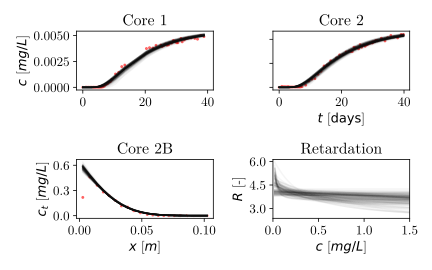
\includegraphics{figs/finn_fullspan_samples.pdf}
    \caption{Retardation samples and correspoding concentration curves obtained from it by training FINN with random hyperparameters and random datasets using PI3NN.}
    \label{fig:fullspan_samples}
\end{figure}



\subsection{HyDa-NNPIE vs. MCMC}

\paragraph{Baseline (Bayes NN via MCMC)}
We computed $10$k samples using the same parameters as \cite{finn}; the samples are visualized in Figure ~\vref{fig:mcmc_samples}.
% TODO: Why 10k? This is very important to know for arguing about efficiency.

\begin{figure}[h!]
    \centering
    \includegraphics{figs/finn_mcmc_samples.pdf}
    \caption{Retardation factors generated by MCMC sampling as detailed in Section ~\vref{sec:bayes_nn}.}
    \label{fig:mcmc_samples}
\end{figure}


\paragraph{Retardation Factor Uncertainty Comparison}
Figure ~\vref{fig:mcmc_vs_fullspan} illustrates that the 90\% PIs for both the MCMC and HyDa-NNPIE methods encompass similar concentration values. This agreement arises from their comparable coverage of $R(c)$ values when $c \leq 1$. While the methods diverge for larger values of $c$, this discrepancy has minimal impact on the concentration fields, as these are less sensitive to $R(c)$ in that regime. Given that HyDa-NNPIE produces similar $c$ PIs but incorporates larger uncertainty in $R$, it provides a more robust uncertainty estimate. A more quantitative exploration of these findings is presented in the following sections.

\begin{figure}[h!]
    \centering
    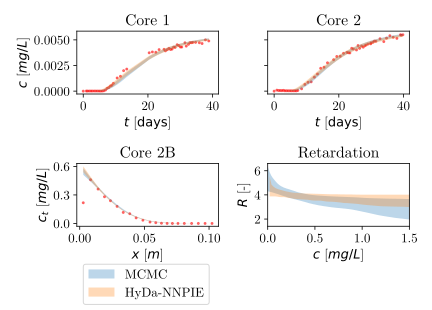
\includegraphics{figs/finn_MCMCvsFull-SPAN_PIs.pdf}
    \caption{Retardation PIs and correspoding concentration PIs obtained from it by training FINN with random hyperparameters and random datasets using PI3NN (orange). Compared with MCMC approach (blue). (90\% PIs are depicted.)}
    \label{fig:mcmc_vs_fullspan}
\end{figure}




\paragraph{Runtime Comparison}
We measure and compare the runtime of generating a single sample of our method and the baseline. Since NNPIE requires training of the NN from scratch for each sample, the runtime approximately equals the training time. Averaging over $10$ trials, the runtime is $170$ seconds.

The MCMC method uses thinning, saving only every $10$th sample. The average runtime for this is about $11.4$ seconds, almost $15$ times faster than our method as also seen in Figure \vref{fig:runtime_comparison}.
However, when considering the total number of samples used for both methods, our method is about $10$ times faster.
% TODO: But how many samples does each method need?
% TODO: And what if the log posterior trace plot is still decreasing? Am I even allowed to take samples from it then?
% TODO: What about parallelization? Our method is trivially paralellizable. What about MCMC with Barker sampler?
% TODO: What about other problems (with e.g. more weights). Does our method get better then?

\begin{figure}[h]
    \centering
    \includegraphics{figs/runtime_comparison.pdf}
    \caption{Runtime for generating a single sample (left panel) and all samples (right panel) using NNPIE (left bar) and MCMC (right bar). Measured on the same machine and averaged over $10$ trials.}
    \label{fig:runtime_comparison}
\end{figure}



\paragraph{Likelihood Comparison}
\label{sec:likelihood}
To evaluate the predictive quality of our method, we use its samples to estimate a probability distribution. This is done by computing a histogram. We can then estimate the likelihood of the training data $\mathcal{D}$ given this distribution. We transform the likelihood into a negative log-likelihood (NLL) to obtain more accurate results. A lower NLL is better. Applying this procedure on Hy-NNPIE yields a NLL of $-6.41$, $-7.11$ for MCMC, and $-7.14$ for Da-NNPIE. A good baseline to compare this against, is a normal distribution around the FINN BTC prediction mean and standard deviation equal to the sample standard deviation computed from the residuals:
\begin{equation*}
    p(c; t) = \frac{1}{\sqrt{2 \pi \mathcal{s}^2}} \exp(-\frac{1}{2 \mathcal{s}^2} (\hat{c}(x=L, t; \theta_{\mathcal{D}}) - c)^2)
\end{equation*}
This yields a NLL of $-7.50$, which is the lowest value. % TODO: Interpretation



\paragraph{PI Calibration Comparison}
Another quantification done by \cite{finn} is the average calibration of the PI. This can be visualized using the reliability curve.

The reliability curve assesses the calibration of predicted confidence intervals. It plots the observed frequency of the true value falling within a given confidence interval against the predicted confidence level. To compute it, the prediction range is divided into bins (e.g., by confidence levels). For each bin, the proportion of predictions where the true value falls within the corresponding PI is calculated. Ideally, the curve should follow the diagonal line (perfect calibration). A curve above the diagonal indicates underconfidence (the true value falls within the PI more often than predicted), while a curve below the diagonal indicates overconfidence.

The results, shown in Figure ~\vref{fig:reliability_curves}, suggest that Da-NNPIE provides the best calibrated PI. Overall, all methods are generally overconfident, Hy-NNPIE the strongest. Only Da-NNPIE is a little underconfident for very small $c$ values.

\begin{figure}[h]
    \centering
    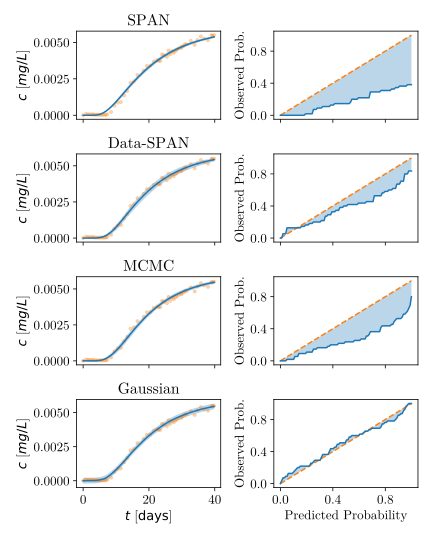
\includegraphics{figs/reliability_curves.pdf}
    \caption{Top: Core 2 BTC 90\% PIs for the different methods (Hy-NNPIE, Da-NNPIE, MCMC). Bottom: Reliability curve for each method.}
    \label{fig:reliability_curves}
\end{figure}


\section{Summary}
The analysis of our results reveals several key insights regarding the performance and characteristics of the different uncertainty estimation methods, particularly focusing on the comparison between HyDa-NNPIE and MCMC.

Firstly, the synthetic data case exhibits significantly lower uncertainty compared to the experimental data scenario. This can be attributed to several factors: a larger number of datapoints, which reduces epistemic uncertainty; the reduced effectiveness of Da-NNPIE due to the absence of real noise and presence of artificial noise in the synthetic data, which, although introducing some level of uncertainty, does not represent a real distribution, rendering the application of PI3NN, our strongest method to generate datasets, unreasonable since it is designed to learn the underlying real distribution; and the utilization of less effective hyperparameters (such as excluding the strongest options like \textbf{Number of Epochs} or \textbf{MSE loss factor}, as shown in Section ~\vref{sec:sensitivity}).

Given that the hyperparameters Hy-NNPIE have a negligible impact on output variation relative to Da-NNPIE, and considering Da-NNPIE's ability to efficiently sample the entire space due to its one-dimensional nature, HyDa-NNPIE requires substantially fewer samples than MCMC. This is a favorable characteristic, as it implies that HyDa-NNPIE can achieve reliable uncertainty estimates even with a limited number of samples and thus computational effort. Furthermore, HyDa-NNPIE benefits from trivial parallelizability, unlike MCMC, which requires sequential sampling or more advanced methods. This, coupled with the ability to operate effectively with fewer samples, establishes HyDa-NNPIE as a more computationally efficient method for UQ.


% TODO: Btw, I remember that I was told not to use the word "parameter" because this can be confused with something else.








\chapter{Conclusion}
\label{sec:conclusion}
Although our sensitivity analysis indicated that certain hyperparameters exerted minimal influence on the results, their inclusion does not negatively affect performance. This is because Monte Carlo sampling, the core technique employed here, is inherently independent of dimensionality.

Finally, a comparison of the PIs generated by HyDa-NNPIE and MCMC, specifically the $R(c)$ PI, and their respective likelihoods, reveals comparable performance. Qualitatively, both methods appear to achieve a similar level of accuracy in capturing uncertainty.


\section{Limitations}
One limitation of our approach lies in its ``brute-force'' nature, due not only to the computational effort but also to the process itself. While we gain insights into uncertainty, the obtained result is highly dependent on the used solver and selected hyperparameters in the case of Hy-NNPIE and highly dependent on the given dataset in the case of Da-NNPIE. Ideally, uncertainty is a byproduct of the method and the uncertainty in the data.

Furthermore, the weighting process raises concerns. The BTC is constrained to a small subset of concentration values compared to the entire field (only 0 to 0.04 instead of 0 to 1.0). This raises questions about the validity of weighting, e.g. $R(c=0.0)$ samples the same way as $R(c=1.0)$, as the latter do not directly influence the predicted BTC and thus their likelihood contribution is questionable.

While the empirical investigation into the uniqueness of the retardation factor $R(c)$ provides valuable insights, it has several limitations. First, the study is based on synthetic datasets generated using known parametric isotherms (Langmuir, Freundlich, and linear). This limits the generalizability of the findings to real-world scenarios where the retardation factor might follow different, potentially more complex functional forms. Second, the numerical approximation of derivatives using a B-spline surrogate model introduces some degree of error, which could affect the accuracy of the estimated $R(c)$ values, as seen by the noise in the raw estimates. While we addressed this through binning and averaging, the choice of bin size could influence the results, and some information loss is inevitable. Finally, the empirical nature of the investigation means that it cannot provide a formal mathematical proof of uniqueness, but rather suggestive evidence within the confines of the tested scenarios. Further theoretical analysis would be needed to definitively establish the uniqueness of the inverse problem for a broader range of conditions.


\section{Summary and Outlook}
This work investigated UQ for the retardation factor in a diffusion-sorption process using the FINN framework. We proposed two novel UQ methods, Hy-NNPIE and Da-NNPIE, based on perturbing hyperparameters and training data, respectively. Empirical analysis demonstrated the near uniqueness of the inverse problem, enabling interpretation of the UQ results. Although computationally more expensive than MCMC, our methods offer a different perspective on uncertainty by directly exploring the effects of various uncertainties within the training data and solver process.


\subsection{Outlook}
While the presented results are promising, several avenues for future research exist.

One direction is the development of more efficient and scalable UQ methods for FINN. While NNPIE offers advantages in terms of parallelizability and sample efficiency compared to MCMC, it still relies on training multiple instances of FINN, which can be computationally demanding for large-scale problems. Exploring techniques like dropout or other kinds of ensemble learning could help reduce the computational burden.

Furthermore, investigating the applicability of NNPIE to other types of PDEs and inverse problems is an important direction. The core principles of marginalizing over hyperparameters and data uncertainties are general and could be adapted to other settings. However, the specific implementation details, such as the choice of hyperparameters and the data sampling techniques, might need to be tailored to the specific problem at hand.

Additionally, while this study focused on UQ for the retardation factor, extending the analysis to other uncertain parameters or model components within the FINN framework is a valuable direction.

Finally, a more rigorous theoretical analysis of the proposed UQ methods would be beneficial. This could involve investigating the convergence properties of the Monte Carlo estimators, deriving error bounds, or exploring the connections to existing UQ frameworks like Bayesian inference.




% TODO: I miss \textcite...
% TODO: Justify hyperparameter ranges.
% TODO: How where PI3NN Hyperparameters chosen?



% TODO: Include this in experiments section
% \begin{figure}[h]
%     \centering
%     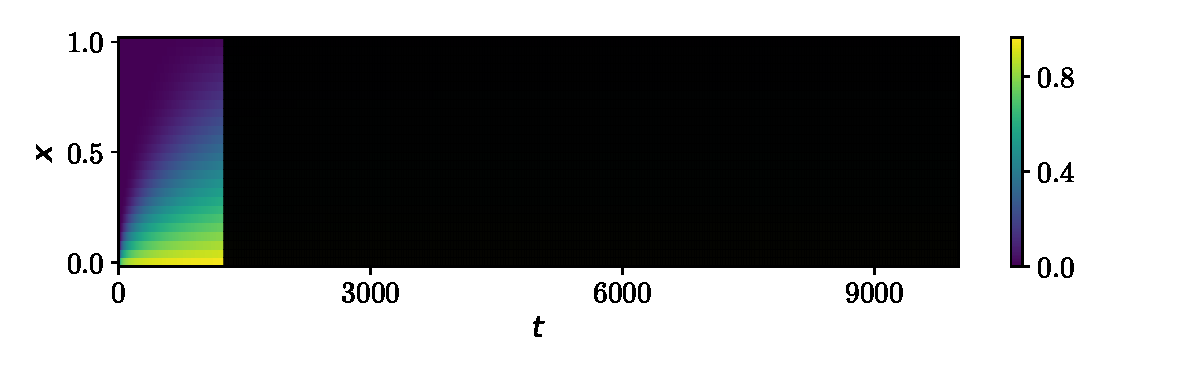
\includegraphics{figs/c_diss_field_full_black_test.pdf}
%     \caption{Training data for the model, represented by a pcolor plot of the synthetic concentration field $c(x,t)$ generated using the Langmuir isotherm. The spatial domain is $x \in [0, 1]$ meters, and the temporal domain is $t \in [0, 10000]$ days. The period from $t = 1255$ to $t = 10000$ days is masked, indicating that these values are not used for training but are reserved for testing.}
%     \label{fig:c_diss_field_full_black_test}
% \end{figure}




\section*{Appendix}


\subsection*{Retardation Range} % is this an Ablation Study? % TODO: better name?
It is observed that $R(c)$ does not affect the entire $c$ field uniformly. This can be illustrated by examining Figure ~\vref{fig:triangle_ret_pertubation}, which depicts constant retardation factors perturbed additively by triangle functions centered at different $c$ values. As the center of the triangle function increases, the error caused by the perturbation rapidly diminishes and becomes zero for $c > 1$. This is because the concentration field $c(x,t)$ is bounded between 0 and 1. Furthermore, there is a notable discrepancy between the maximum error measured over the full field and the error measured in the breakthrough curve (BTC). The BTC error is consistently lower than the full field error.

However, in the case of experimental data, the full field error cannot be detected, as the full field solution is not accessible. Consequently, the range of $c$ values for which meaningful statements can be made about the uncertainty of $R(c)$ is limited to a narrow range. The exact extent of this range is difficult to estimate, as the strength of influence of different retardation factors is not well understood.
As a result, we restrict our analysis and plotting of $R(c)$ to the range $0 \leq c \leq 1.5$, whereas the comparable study by Finn \cite{finn} presents results over the range $0 \leq c \leq 2.0$.


\begin{figure}[h]
    \centering
    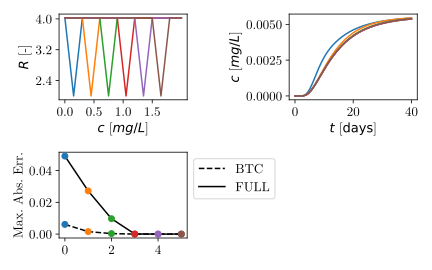
\includegraphics{figs/triangle_ret_pertubation.pdf}
    \caption{Left: Retardation factors with triangle peaks. Middle: Concentration BTC for these retardation factors. Right: MAE for each on the full field and BTC.}
    \label{fig:triangle_ret_pertubation}
\end{figure}